\documentclass[ngerman,pstricks,border=12pt]{standalone}
% --- Pakete einbinden
\input{01_PaketeEinstellungen.tex}
\begin{document}
\setcounter{figure}{9}
\begin{figure}[H]
\centering
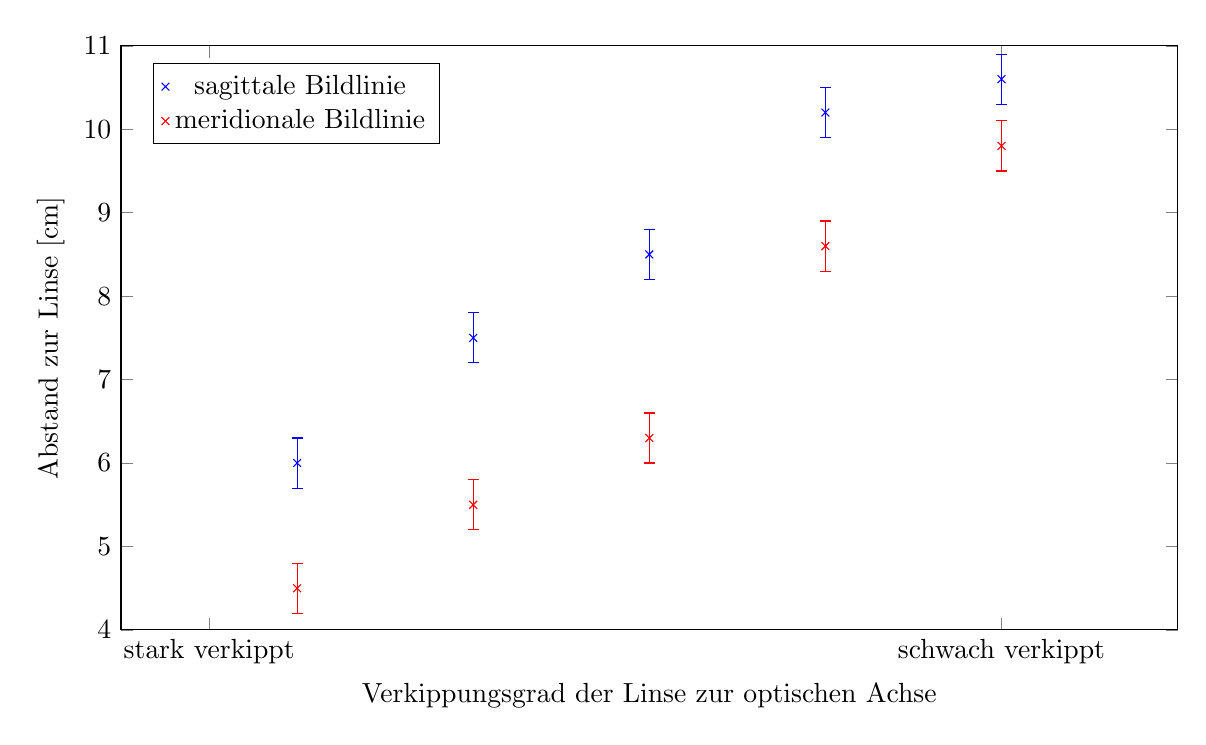
\begin{tikzpicture}
  \begin{axis}[
    width=15 cm,
    height=9 cm,
    xmin=0, xmax=6,
    ymin=4, ymax=11,
    xlabel={Verkippungsgrad der Linse zur optischen Achse},
    ylabel={Abstand zur Linse [\si{cm}]},
    domain=-3:17,
		xtick={0.5,5},
		xticklabels={stark verkippt, schwach verkippt},
    legend entries={sagittale Bildlinie, meridionale Bildlinie},
    legend pos=north west
  ]
  \addplot+ plot [only marks,mark=x, error bars/.cd, y dir=both, y fixed=0.3]  coordinates {
		(1,6.0) (2,7.5) (3,8.5) (4,10.2) (5,10.6)
	};
	\addplot+ plot [only marks,mark=x, error bars/.cd, y dir=both, y fixed=0.3]  coordinates {
		(1,4.5) (2,5.5) (3,6.3) (4,8.6) (5,9.8)
	};
	\end{axis}
\end{tikzpicture}

\label{fig:astigma}
\end{figure}
\end{document}